\chapter{Introduction}

The challenges in powering LED loads are so relevant that have an impact in functionalities and design of the future \emph{Solid-State-Lighting} (SSL) products. So much, that the user adoption of such a beneficial technology by is far slower than comparable disruptive technologies~\cite{11Voger}. In a part, that could be attributed due to the difficulties in achieving the high miniaturization and performance necessary in the LED drivers, at low cost, in order to outcompete the cheaper old technologies.

From the power management standpoint power a LED load is a trivial task, however the different requirements of SSL products make the design of them a complex task. Initially the main driving forces in the driver designs where: manufacturing cost, power quality, light quality. Reducing manufacturing costs can enable to decrease the lamp prices to the entry point for the consumers. The drivers have to fulfill with the legislation in terms of power quality not exceeded the minimum \emph{Power Factor} (PF) and \emph{Total Harmonic Distortion} (THD). From the consumer point of view the light quality is measured in terms of: flickering, color consistency and \emph{Color Rendering Index} (CRI), being the flickering a parameter related to the driver design. Flickering must be kept  under certain limits to do cause health concerns~\cite{10Wilkins}.
Recently two other factors are becoming more relevant in the driver: miniaturization and  controllability. The volume of the drivers is currently, in many cases, limited by the old lamp shapes in order to provide retrofit solutions. There are solutions for all incandescent lamps, however there are still challenged for small halogen cases. Anyway the miniaturization requirements of the lamps have been relaxed by redefining the shape and look of the old lamps, the new design take large part of the lamp volume for the heat sink body, what allows a large volume for the driver. Further reduction of the driver will enable higher freedom in the lamp design. The future connected lamps~\cite{14Harbers} will require control and connectivity, what challenges the driver to provide multiple color channels, current control and power management for added intelligent circuitry such as MCUs and sensors.

The high and diverse level of requirements for the LED drivers has made the design process a complex task, further than just a pure power management problem. The initial driving forces in driver design, cost, power and light quality, found effective solutions  based on discrete components.  The new driving forces where miniaturization, controllability and connectivity brings to research in the context of \emph{Power Systems on-Chip/in-Package}(PSoC/PSiP), where miniaturization and integration of functionalities can be easily achieved. This chapter starts with an analysis of the LED characteristics to understand why is a driver necessary. Subsequently, the three different driver technologies are studied: Linear, switched inductor converters and switched capacitor converters. An state-of-the-art for each technology will be provided in order to construct a rational of the technology toward miniaturization. Switched capacitor converters will be thoroughly studied, since constitute the central conversion technology selected for this dissertation.


\section{The LED load}
\label{sc:LED_load}
The LED is just a special diode that emits light as the acronym stands for \emph{Light Emitting Diode}. It is well known that a diode has a very \emph{voltage-current} ($v-i$) curve as shown in Figure~\ref{fig:led_I-V}. For voltages below the \emph{forward voltage}, $v_{f}$, there is practically no current flow and the LED behaves as an open circuit. The same characteristic applies  when reversed bias until the breakdown voltage, $v_{break}$, is reached. For voltages above $v_{f}$ the curve becomes very steep and the current increases dramatically with respect to the voltage, thus the LED behaves as a short circuit. The similar behaviour happens when the LED is reverse biased and the voltage is above $v_{break}$, however in this case there is no light generation. The LED has to be supplied at an specific point $P$ in order to provide a desired light output as shown in Figure~\ref{fig:led_I-V}, depending on the bias current light colour and intensity will vary. Due to the steepness in the $v-i$ curve, the practical way to bias a LED is supplying them with a \emph{dc}-current. Since the common used energy sources are voltage supplies, it is necessary to select a circuit that converts the input energy from the voltage source to a constant current.

\begin{figure}[!h]
\centering
\begin{circuitikz}[american voltages]

    \draw (0,2.5) to[leD*,v=$v$,i=$i$,*-*] (3
    ,2.5) ;

\begin{scope}[xshift=4cm, domain=0:6]
    \draw [->] (0,0) -- (5.5,0) node[anchor=west]{$v$};
    \draw [->] (0,0) -- (0,5.5) node[anchor=east]{$i$};

    %Mark Vth
    \draw (2,2pt) -- (2,-5pt) node[anchor=north] {$v_{f}$};

    %Mark Vthmin and Vt_max
    \def\dvf{0.25}
    \def\dvftop{0.45}

    \draw (1.5,2pt) -- (1.5,-5pt) node[anchor=north] {};
    \draw (2.5,2pt) -- (2.5,-5pt) node[anchor=north] {};
    \draw[dotted] (1.5,0) -- (1.5,\dvftop);
    \draw[dotted] (2.5,0) -- (2.5,\dvftop);
    %Mark Delta Vf
    \draw[pil,>-< ,dotted] (1.25,\dvf) -- (2.75,\dvf);
    \draw (1,\dvf) -- (1.5,\dvf) node[anchor=south east] {$\Delta v_f$};


    %Draw ideal plot
    \draw[thick] (0,0) -- (2,0) -- (4.5,5);

    %Draw lower limit
    \draw[dashed] (0,0) -- (1.5,0) -- (4,5);
    %Draw higher limit
    \draw[dashed] (0,0) -- (2.5,0) -- (5,5);

    %Draw bias point projection
    \draw[dotted] (4,4) -- (4,-0);
    \draw (4,2pt) -- (4,-5pt) node[anchor=north]  {$v_{bias}$};

    \draw[dotted] (4,4) -- (-0,4);
    \draw (2pt,4) -- (-5pt,4) node[anchor=east]  {$i_{bias}$};

    %Draw bias point
    \filldraw (4,4) circle(2pt) node[anchor=south west] {$P$};

    %Draw bias point variations
    \draw (4.5,4)  node[anchor=south west] {};
    \draw (3.5,4)  node[anchor=south west] {};

    %\draw[loosely dotted] (4.5,4) -- (4.5,-0);
    %\draw[loosely dotted] (3.5,4) -- (3.5,-0);
    \draw (4,2pt) -- (4,-5pt) node[anchor=north]  {$v_{bias}$};
    %Mark Vthmin and Vt_max
    \def\bpmi{4.5}
    \def\bpMa{3.5}
    %\draw (1.5,2pt) -- (1.5,-5pt) node[anchor=north] {};
    %\draw (2.5,2pt) -- (2.5,-5pt) node[anchor=north] {};
    %\draw[dotted] (1.5,0) -- (1.5,\dvftop);
    %\draw[dotted] (2.5,0) -- (2.5,\dvftop);
    %Mark Delta Vf
    %\draw[pil,>-< ,dotted] (3.25,\dvf) -- (4.75,\dvf);
    %\draw (4.5,\dvf) -- (5,\dvf) node[anchor=south west] {$\Delta V_{bias}$};

    %Mark Vthmin and Vt_max
    \def\dvf{4}
    %\draw (1.5,2pt) -- (1.5,-5pt) node[anchor=north] {};
    %\draw (2.5,2pt) -- (2.5,-5pt) node[anchor=north] {};
    %\draw[dotted] (1.5,0) -- (1.5,\dvftop);
    %\draw[dotted] (2.5,0) -- (2.5,\dvftop);
    %Mark Delta Vf
    \draw[pil,>-< ,dotted] (3.25,\dvf) -- (4.75,\dvf);
    \draw (4.5,\dvf) -- (5,\dvf) node[anchor=south west] {$\Delta v_{bias}$};


\end{scope}
\end{circuitikz}
\caption{Idealized LED voltage-current characteristic, with the \emph{forward voltage} $v_f$  identified and a projection of the \emph{bias point} P }
\label{fig:led_I-V}
\end{figure}

At first glance, keeping a constant bias current, $i_{bias}$, through the LED does not seems to be challenging, however the LED's electrical characteristics are not static and have some tolerances. On the one hand, a LED has different sources of deviations that the driver circuit has to deal with them in order to keep them delivering the desired light output. First, $v_f$ has a negative dependence with the temperature, drooping its values as the \emph{pn}-junction temperature increases. Second, the LED has an aging factor which derates the light output over time, and which has to be adjusted by changing the bias point. And last, during production LEDs will vary in colour, flux, and forward voltage; even for products from the same batch. The manufacturers have reduced the tolerances between devices by binning \footnote{Quality control performed at LED production line, where each LED is individual tested and sorted in groups (bins) that have the same electrical and lighting characteristics.}, but after binning, the parts suffer deviations, \emph{e.g.} up to $10\%$ in $v_f$. Figure ~\ref{fig:led_I-V} shows graphically how deviations in $v_f$ produce a displacement in the $v-i$ characteristic,  which require to modify the $v_{bias}$ within a certain range $\Delta v_{bias}$ in order to keep $i_{bias}$ constant. On the other hand, the voltage provided by the energy supply has some tolerances. Depending on the nature of the energy supply, \emph{ac} or \emph{dc}, the driver has to provide line regulation, filter high frequency perturbations and accept the voltage tolerances of the source, without affecting the light output. In general, LEDs lamps have to provide a certain desired light output range despite variations in the LED characteristics or the voltage supply, and therefore that control function is what adds complexity to the driver circuit. The three families of LED drivers will be presented in the subsequent sections.

\section{Linear Regulators}
Linear drivers place a shunt element between the source and the load(\emph{i.e} the LED). The shunt element limits the LED current providing the necessary voltage droop between the source and the load. The excess of voltage between the source and the load is dissipated in the series element, literally burned in form of heat; therefore these drivers become very inefficient if the LED voltage is not close to the source. Other limitation is that linear drivers only provide step-down conversion, thus they cannot work when the voltage at the load is higher than the input supply.

\begin{figure}[!h]
\centering
\ctikzset { bipoles/length=1cm}
\begin{subfigure}[t]{.45\textwidth}
    \centering
    \begin{circuitikz} [american voltages,scale=0.65]
    \draw
        (0,0) to[V = $v_{src}$]
        (0,3) to[generic=$r_series$,i=$i_o$]
        (5,3) to[leD*,v=$v_{o}$]
        (5,0) -- (0,0);
    \end{circuitikz}
    \caption{}
    \label{fig:linear_ckt}
\end{subfigure}
\begin{subfigure}[t]{.45\textwidth}
    \begin{circuitikz} [scale=0.65]
    \begin{scope}%[xshift = 8cm, yshift=0cm]
        \draw[->] (0,0) -- (4,0) node[anchor=south] {$  m $};
        \draw[->] (0,0) -- (0,3.2) node[anchor=east] {$\eta $};

        %Ticks X
        \draw (3,-5pt) -- (3,2pt)  node[anchor=south west] {$1$};
        \draw (1.5,-5pt) -- (1.5,2pt)   node[anchor=south west] {$0.7$};

        %Ticks Y
        \draw (2pt,2.5) -- (-5pt,2.5) node[anchor=east] {$100\%$};
        \draw (2pt,1.5) -- (-5pt,1.5) node[anchor=east] {$70\%$};

        %Markers
        \draw[dotted] (3,2.5) -- (3,0);
        \draw[dotted] (3,2.5) -- (0,2.5);
        \draw[dotted] (1.5,1.5) -- (1.5,0);
        \draw[dotted] (1.5,1.5) -- (0,1.5);


        \draw[thick] (3,2.5) -- (0,0.5);
    \end{scope}
    \end{circuitikz}
    \caption{}
\label{fig:linear_chr}
\end{subfigure}
\caption{Linear driver, \emph{left}- schematic; \emph{righ}- conversion ratio vs. efficiency characteristics}
\label{fig:linear_drv}
\end{figure}

The circuit of the Figure~\ref{fig:linear_ckt} shows the schematic of a linear driver. The shunt element can be implemented with just a resistor of with an active device. The first will impose a current depending on the input source and the load conditions; the second will provide regulation of the bias point for variations in the source and in the load. Linear drivers are very simple to implement, with very low costs and taking almost no volume, being indeed the perfect solution for integration since they do not make use energy storage components for power processing.

The plotted graph in Figure~\ref{fig:linear_chr} presents the variation of the driver efficiency with respect to the conversion ration $m$. Here $m$  is the ratio between the input voltage, $v_{src}$,  and the output voltage,$v_o$, being defined as
   \begin{equation}
        m = \frac{v_o}{v_{src}}.
   \end{equation}

The efficiency of the driver is the ratio between the input power and the output power
   \begin{equation}
        \eta = \frac{P_o}{P_i} = \frac{v_o i_o}{v_{src} i_o} = \frac{v_o}{v_{src}},
   \end{equation}

hence for this case the efficiency is indeed equal to the conversion ratio
   \begin{equation}
        \eta = m.
   \end{equation}
Owing to the fact that LED drivers have to be efficient, and assuming that a worst case 80\% efficiency can be accepted, linear drivers could only be suitable where the ration between input voltage and load voltage is higher than 0.8.


\section{Inductor Based Converters}

\emph{Inductor Based Converters} (IBCs) are \emph{Switched Mode Power Supplies} (SMPS) \footnote{Electronic power supply that provides efficient electric power conversion by commuting between different circuit configurations (modes).}  that employ magnetic passive elements (i.e. inductors and transformers) to store energy and provide efficient electrical power conversion. Since IBCs are very efficient with respect to voltage-to-current conversion, they are ideal as LED drivers.

The inductor is the main element in these converters and it allows voltage conversion by storing energy in form of magnetic field. In the case of the converter of the figure~\ref{fig:induct_ckt} the inductor is charged during

These converters can provide step-up and step-down conversion for large dynamic ranges while keeping the efficiency very high. On top of their power conversion capabilities, such converters can also provide galvanic isolation, which in many applications is compulsory in order to guarantee the safety of the users against electrical hazards. Such characteristics suggest these drivers as the preferred solution for the LED industry. Figure~\ref{fig:induct_ckt} shows one of the most popular implementations for LED drivers: The \emph{buck} converter.  Figure~\ref{fig:induc_chr} presents the regulation characteristic of a generic  inductor based converter. As shown, the theoretical efficiency of these converters is 100\% for all the conversion ratio range. In practice, due to parasitics in switches and inductors, the efficiency drops to a certain value with small fluctuations with respect to the conversion range.

\begin{figure}[!h]
\centering
\ctikzset { bipoles/length=1cm}
\begin{subfigure}[t]{.45\textwidth}
    %\centering
    \raggedright
    \begin{circuitikz} [american voltages,scale=0.65]
    \draw
        (6.5,0) to[short]
        (0,0) to[V = $v_{src}$]
        (0,3) to[switch]
        (3,3) to[inductor=${L}$,i=$i_o$]
        (6.5,3);

    \draw (2.5,3) to[switch] (2.5,0);

    \draw (6.5,3) to[leD*,v=$v_{o}$] (6.5,0);

    \end{circuitikz}
    \caption{}
    \label{fig:induct_ckt}
\end{subfigure}
\hfill
\begin{subfigure}[t]{.45\textwidth}
    %\centering
    \raggedleft
    \begin{circuitikz} [scale=0.65]
    \begin{scope}%[xshift = 8cm, yshift=0cm]
        \draw[->] (0,0) -- (4,0) node[anchor=south] {$  m $};
        \draw[->] (0,0) -- (0,3.2) node[anchor=east] {$\eta $};

        %Ticks X
        %\draw (3,2pt) -- (3,-5pt) node[anchor=north] {$1$};
        %\draw (1.5,2pt) -- (1.5,-5pt) node[anchor=north] {$0.7$};

        %Ticks Y
        \draw (2pt,2.5) -- (-5pt,2.5) node[anchor=east] {$100\%$};
        \draw (2pt,1.5) -- (-5pt,1.5) node[anchor=east] {$90\%$};

        %Markers
        % \draw[dotted] (3,2.5) -- (3,0);
        \draw[dotted] (3,2.5) -- (0,2.5);
        %\draw[dotted] (1.5,1.5) -- (1.5,0);
        \draw[dotted] (1.5,1.5) -- (0,1.5);


        \draw[thick] (0.5,2.5) -- (3,2.5) node[anchor=south] {$Theoretical$};
        \draw[thick,dashed] (0.5,1.20) parabola[bend at end] (3,1.7) node[anchor=north] {$Real$};
    \end{scope}
    \end{circuitikz}
    \caption{}
\label{fig:induc_chr}
\end{subfigure}
\caption{Inductor based converter, \emph{left} - buck converter schematic; \emph{right} - conversion ration \emph{vs.} efficiency curve comparing the \emph{theoretical} and a \emph{practical} limit. }
\label{fig:inductive_smps}
\end{figure}

One of the disadvantages of these converters is the magnetic components, and the volume related to them. In practice, inductors dominate the entire volume of the LED drivers as shown in Figure~\ref{fig:smps_driver}. Integrated implementations of these converters suffer the challenges of using integrated magnetic components. The present \emph{very-large integration scale} (VLSI) technologies do not yet offer power inductors in the commercial implementations, and other integrated inductors are not yet mature enough for non-research products.

Yet another disadvantage for integration is the voltage stress in the switches of the converter. Switches in inductive converters have to withstand the full operational voltage, which depending on the application range, is from tens to a few hundreds of volts. Using high voltage devices has three main drawbacks: First, the losses in the devices scale quadratically with the voltage  stress. Second, bad switching performances, because high voltage devices are less efficient and slower switching. Third, the standard VLSI technologies do not offer these \emph{high voltage} (HV) devices and the VLSI technologies that offer them are less performant and more expensive than the dedicated discrete technologies.

\begin{figure}[!h]
\centering
\begin{tikzpicture}
\node[anchor=south west,inner sep=0] (image) at (0,0) {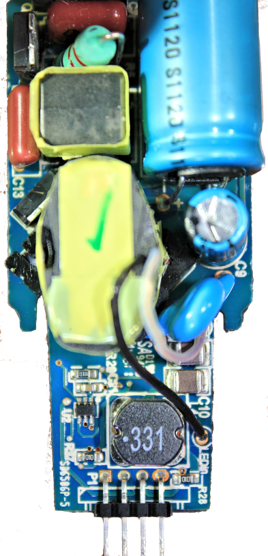
\includegraphics[height=5cm,angle=90]{./0_intro/img/LED_driver.png}};
\begin{scope}[x={(image.south east)},y={(image.north west)}]
%\draw [<-,thick] (0.75,0.5) -- (0.855,0.7)  node [anchor=south west] {Power Magnet};
\draw[black,ultra thick,rounded corners] (0.70,0.3805) rectangle (0.855,0.7);
\draw[black,ultra thick,rounded corners] (0.11,0.1) rectangle (0.28,0.50);
\draw[black,ultra thick,rounded corners] (0.28,0.1) rectangle (0.63,0.62);
\end{scope}
\end{tikzpicture}
\caption{Magnetic components marked with a black square in a mains connected LED driver. These components dominate the volume of the converter.}
\label{fig:smps_driver}
\end{figure}


\section{Capacitor Based Converters }
Switched Capacitor Converters (SCCs) are SMPS composed only of switches and capacitors. SCC were initially used for voltage multiplication~\cite{30Cockcroft,44Waidelich,76Dickson} and more recently in applications that need voltage regulation as well~\cite{Ng:EECS-2011-94}. Compared to inductor based converters, the absence of magnetic elements places them in a good position for high density power systems and integrated solutions, such as Power-System-in-Package (PSiP) or Power-System-on-Chip (PSoC).

SCCs have a fixed ratio of conversion between the input and the output determined by the topology. The output voltage of the converter under no load conditions is defined as the \emph{target voltage} $v_t$. The converter performs at high efficiency when the load is supplied close to the \emph{target voltage}. Similar to the linear drivers, if the output voltage goes below the \emph{target voltage} the efficiency drops and when the output voltage is above the \emph{target voltage} the converter cannot operate. Figure~\ref{fig:SCC_ckt} shows a step-down converter with a conversion ratio of one half.

A common practice to extend the regulation margins of these converters is to have topologies with multiple conversion rations~\cite{2013Ma,2013Breussegem:m_trg}. From Figure~\ref{fig:SCC_chr} it can be seen that the efficiency increases as the ration $m$ gets close to the first fixed conversion ration of the converter $m_1$; right after $m_1$ the efficiency drops again dramatically and it again linearly increases as it approaches the second fixed conversion ratio of the converter $m_2$. Beyond $m_2$ the converter does not work.


\begin{figure}[!h]
%\centering
\ctikzset { bipoles/length=1cm}
\begin{subfigure}[t]{.45\textwidth}
    %\centering
    \raggedright
    %\raggedleft
    \begin{circuitikz} [american voltages,scale=0.65]
    \draw
        (6.5,0) to[short]
        (0,0) to[V = $v_{src}$]
        (0,3) to[switch]
        (2,3) to[capacitor=${c_1}$]
        (3,3) to[switch]
        (5,3) to[short]
        (6.5,3);

    %Parallel switch to ground
    \draw (3.25,3) to[switch] (3.25,0);

    %Switch branch to load
    \draw (1.75,3) --
          (1.75,4.5) to[switch]
          (5,4.5) --
          (5,3);

    %Load and capacitor C2
    \draw (5,0) to[capacitor=$c_2$,-*] (5,3);
    \draw (6.5,3) to[leD*,v_=$v_{o}$] (6.5,0);

    \end{circuitikz}
    \caption{}
    \label{fig:SCC_ckt}
\end{subfigure}
\hfill
\begin{subfigure}[t]{.45\textwidth}
    %\centering
    \raggedleft
    %\raggedright
    \begin{circuitikz} [scale=0.65]
    \begin{scope}[xshift = 10cm, yshift=0cm]
            \draw[->] (0,0) -- (4,0) node[anchor=south west] {$  m $};
            \draw[->] (0,0) -- (0,3.2) node[anchor=east] {$\eta $};

            %Ticks X
            \draw  (1.75,5pt) -- (1.75,0pt) node[anchor=south west ] {$m_1$};
            \draw  (3,5pt) -- (3,0pt)   node[anchor=south west ] {$m_2$};
            %\draw (1.5,2pt) -- (1.5,-5pt) node[anchor=north] {$0.7$};

            %Ticks Y
            \draw (2pt,2.5) -- (-5pt,2.5) node[anchor=east] {$100\%$};
            \draw (2pt,1.5) -- (-5pt,1.5) node[anchor=east] {$90\%$};

            %Markers
            \draw[dotted] (1.75,2.4) -- (1.75,0);
            \draw[dotted] (3,2.3) -- (3,0);
            \draw[dotted] (3,2.5) -- (0,2.5);
            %\draw[dotted] (1.5,1.5) -- (1.5,0);
            %\draw[dotted] (1.5,1.5) -- (0,1.5);


            \draw[thick] (0.5,1.4) -- (1.75,2.4) -- (1.75,1.6) -- (3,2.3)  node[anchor=south] {};
            \draw (10,0)[anchor=north] {};
        \end{scope}
    \end{circuitikz}
    \caption{}
\label{fig:SCC_chr}
\end{subfigure}
\caption{Switched capacitor converter, \emph{left} - 2:1 converter schematic; \emph{right} - conversion ration \emph{vs.} efficiency curve for of a generic multiple  conversion ration stage }
\label{fig:SCC_smps}
\end{figure}

The main advantage of these converters is that they use no inductors, which makes them suitable for integration. Integrated capacitors have a better energy density than integrated inductors. The mechanical structure of the capacitors, a stack of isolator-metal-isolator, is much easier to replicate on a small scale. Yet another advantage of the switch capacitors is that they split the voltage applied to the converter among the different components, thus reducing the voltage stress in the switches and capacitors. Such voltage stress reduction is very interesting from the point of view of integration. First, lower voltage capacitors have better performances: higher energy density, less derating and better chances of integration. Second, lower voltage switches have better switching performances. Finally, low voltage devices take less silicon area and there is more to offer in the standard VLSI technologies, thus reducing the production costs.

The big disadvantage of these converters is that they can not directly provide the voltage-to-current conversion required for the LEDs to work. Nevertheless they are still used as LED drivers in backlighting applications for battery supplied devices. In such cases, the SCCs steps-up or steps-down the battery voltage and afterwards a linear driver  provides current regulation to properly bias the LEDs. Adopting that architecture for general lighting could be a solution, but when  voltages and currents are scaled to the values used in these applications the number of necessary conversion steps of the SCC would make it totally infeasible and inefficient.

Based on the previous arguments adopting an SCC architecture for a general solution for LED drivers seems to be, a priori,  not an evident choice. On the one hand, their limitation in voltage-to-current conversion would directly disqualify switched capacitors. On the other hand, the advantageous characteristics of switched capacitors for integration made these circuits very attractive. Actually, if the initial limitations in voltage-to-current conversion could be overcome, such architecture would be an interesting candidate to explore as a solution for a \emph{Power System on-Chip/in-Package} LED driver.  Exploring the possibilities that switched capacitor converters can offer in terms of integrated and miniaturized LED drivers with efficient voltage-to-current conversion was the rational of this dissertation.


\section{State of the art LED Drivers}
Screen backlighting, Automotive and General Lighting are currently the three main areas of applicaiton of LEDs. Looking into these three areas of application gives a broad overview about the different driver architectures currently used and the approaches towards integration and miniaturization.

With regard to the  miniaturization of power supplies, we can indemnify two clear approaches: \emph{Power System on Chip} (PSoC), and   \emph{Power System in Package} (PSiP). The PSoC approach aims for the integration of the all converter in a single monolithic \emph{Integrated Circuit} (IC). In this approach the power management and the control control circuits are integrated in the same semiconductor die along with energy storage components, with poor energy storage that have on-die inductors and capacitors. The PSiP approach aims for the integration all the necessary functionalities in the same IC package including the passives. This second approach allows to use a large variety of technologies enabling multi-die chips and the integration miniaturized discrete passives in the same package. In line with PSiP, it could be considered a third approach with off-package  passives, and an IC integrating  power management, control and processing.  Actually, this solution is widely spread among the current IC manufacturers regarding power management solutions, however the current solutions only provide the integration of the power train and control circuit or just merely the control circuit.

\citeauthor{2013Breussegem:int_conv}~\cite{2013Breussegem:int_conv} and \citeauthor{2013villar}~\cite{2013villar} provide a comprehensive overview and analysis over the stat-of-art regarding integrated converters, this section provides the overview targeted specific to LED drivers from two points of view application and driver technology.

\subsection{Commercial LED drivers }

Generalist IC manufacturers such as NXP, TI, ST, etc. have a large portfolio of dedicated LED drivers for the this three main applications: Backlighting, Automotive and General Lighting. Innovation from the perspective of the IC manufacturers is very limited just providing the two standard integrated circuit solutions with regard to power management for LED drivers: controller or controller and power train. This approach facilitates the driver development by reducing component count and design time, however  using this circuits the possibilities to reduce the size of the off-chip passives if very limited, topologies are fixed. Currently there is any commercial IC that solves the challenges of the smart drivers, offering connectivity and power management.

Currently the most innovative approach is taken by the startup \emph{Gooee} that proposes connected lighting platform consisting  of two ICs. The control chip integrates a micro-controller unit (MCU) with to implement the communication and sensing, and the power chip with the LED driver that interfaces with the LED; the platform  is completed with a cloud service that enables from a web application to have access to the lamp fixture data logs. The technical details of the power chip are no yet available~\cite{web:Gooee}.

\begin{figure}[t]
    \centering
    \begin{circuitikz} [american voltages,scale=0.65]
    \ctikzset{bipoles/length=0.85cm}
   \draw[thick] (2.5,0.25) --
                (2.5,6.5) --
                (11.5,6.5) --
                (11.5,0.25) --
                (2.5,0.25);

    %Draw SCC block with capacitors
    \draw (3,1) --
          (3,6) --
          (5,6) --
          (5,1) --
          (3,1);

    \draw (4,1.25) node[rotate=90,anchor=west] {Regulator SMPS };

    \draw (5,5.5) to[short,-o] (14,5.5);
    \draw (13,5.5) to[capacitor] (13,4.5) node[sground]{};

    \draw (4,1) -- (4,0) node[sground,scale=0.75]{};

   %Draw linear drivers
   \draw  (4,0.5) -- (10.5,0.5) -- (10.5,1);

   %First transitor
   \draw   (10,1) -- (10,1.5) node[npn,anchor=E,scale=0.5](npn1){}
           (npn1.C) -- (10,2.75) to[short,-o] (12,2.75);

   %Second transitor
   \draw  (10,1) -- (11,1)
           node[npn,anchor=E,scale=0.5](npn2){}
           (npn2.C) -- (11,2.25) to[short,-o] (12,2.25);

   %Controller box
   \draw (5.5,1) -- (8.5,1) -- (8.5,3) -- (5.5,3) -- (5.5,1);
   \draw (5.75,2) node[anchor=west, text width = 1.75cm]{Intensity Controller};
   \draw (npn2.B) -| (8.5,2);
   \draw (npn1.B) -| (8.5,2);

   %LEDs

   \draw [dotted] (14,5.5) to[short,o-] (15,5.5)
                  (15,2.75) to[short,-o] (12,2.75);
                  
   \draw (15,5.5) to[leD*] (15,2.75);

   \draw [dotted] (15,5.5) -- (17,5.5)
                  (17,2.25) to[short,-o] (12,2.25);
                  
   \draw (17,5.5) to[leD*] (17,2.25);

   %Add battery

   \draw (1,0) node[sground,scale=0.75]{};
   \draw (1,0) to[V = $v_{src}$] (1,5.5)
         -- (3,5.5);

    \end{circuitikz}
    \caption{Block diagram of the common architecture used in drivers for backlighting applications.}
    \label{fig:backlight_LED}
\end{figure}

Backlighting for screens in phones, tablets, laptops and TVs was one of the first commercial application of high brightness LEDs (HB-LEDs). Backlighting applications require multiple LED channels, therefore these drivers are generally implemented with a two stage architecture as shown in Figure~\ref{fig:backlight_LED}. The first stage - normally implemented with SMPS, inductive or capacitive-  boosts the supply voltage above the highest voltage of the LED strings. The different strings are individually driven by a linear driver which enables to adjust and dim the currents for each channel individually ~\cite{2008Yuequan,07Feng}. Current commercial solutions integrates power train and power management in a single IC package, using off-chip passives. Drivers for mobile devices, phones and tablets, accept low voltages between 2.5V to 5V, and implement the SMPS stage with an inductive or a capacitive converter. For bigger screens the drivers accept higher voltages between 5V to 45V, and the SMPS stage is normally implemented with an inductive boost converter. In both cases currents are in the low range between between 20mA to 100mA for each string channels, with the exception of the flash light that requires currents burst of up to 1A.

Signaling for the tail lights was the initial application of LEDs in the automotive industry, with the consolidation of the HB-LEDs, LED lighting is currently used also in headlights~\cite{2008Gacio}. Drivers for automotive applications have to deal with a wide range in the input voltage  from 6V to 42V between and provide immunity for the transients in the battery line~\cite{2005mednik,2012Saponara}. The currents change depending on the application, for signaling currents are between 20mA to 100mA, and for head lighting around 1A.  These drivers are implemented  with the popular inductive converters such as Boost, Back, Back-Boost or SEPIC. The available commercial products control ICs using off-chip passives and switches for scalable solutions, or power train and control ICs using off-chip passives. A new trend in the automotive lighting field is the matrix LED technology for headlamps~\cite{web:AUDI_MATRIX}, where a matrix of individually driven LEDs provide high-precision illumination for the drivers, enabling higher safety during night conduction. Matrix LED headlights represent a new challenge for the LED driver, requiring individual control for each of the LEDs in the matrix. The current used architecture connects a switch in parallel of each individual LED, by closing the switches the LEDs can be short-circuited allowing to turn them off or dimming the light intensity ~\cite{2014DS_TI:LED_Matrix_Manger}.

General lighting is currently the main application of high brightness LEDs and the one with the most variants with respect to the drivers. Drivers for general lighting are supplied from the mains utility (\emph{ac} source ) and they require a buffer element in order to provide constant power to the LEDs, which is generally implemented with an electrolytic capacitor. This buffer capacitor is one main contributors in volume and failures, limiting the lamp design and lifetime. Therefore reducing the volume of the capacitor is one of the important aspects in the miniaturizations of off-line drivers, and it can be done by reducing the operating voltage or the required value enabling to use other technologies with better reliability or energy density such us multi-layer ceramics chip capacitors (MCCC) or  thin film plastic capacitors.

Three different architecture approaches are currently implemented in off-line drivers:
\begin{description}
  \item[Single stage] A SMPS, a buck or a fly-back,  converts the input rectified mains voltage to a constant current to supply the LEDs. At the same time the driver keeps the power quality within the standards in terms power factor (PF) and total harmonic distortion (THD). This approach has the advantage of a reduced costs since it has a small number of components, just  requiring one power transistor and one magnetic component. However it is necessary to use a big buffer capacitor in parallel to the LEDs in order to have an stable output voltage and avoid the flickering from the low frequency rectified mains voltage (100Hz - 120Hz).  Currently it is one of the most popular solutions for domestic lighting products for powers up to 70W, and there is a large portfolio of ICs implementing the control or the control and power train, passives have to be used off-chip.

  \item[Two stage] Rectified mains voltage is first converted to a \emph{dc} bus voltage and stored in to the buffer capacitor with almost unity power factor. A second stage converts the power from the buffer capacitor to the LED strings. In this approach the size of the buffer capacitor can be optimized adjusting the voltage and ripple in the bus voltage, which leads to an smaller value than the single stage approach. As a draw back these architecture are more expensive and require double number of components, switches for two power train and at least two different magnetic components. Two stage drivers are used in professional lighting applications, for powers above 100W, and for domestic application for smart bulbs with color tuning, usually both applications require a drivers with  multiple outputs to efficiently supply independent LED strings. There are not dedicated power factor controllers (PFC) ICs  for lighting applications, therefore first stages are just designed and mounted with generic power management ICs for PFC. For the second stage, the IC manufacturer offer a portfolio of drivers for the standard inductive converters (back, boost and flyback),  with the two common options in power management ICs: controller or integrated controller and power train, passives are mounted off-chip.


  \item[Tap linear] Rectified mains is directly supplied two the LEDs by means a matrix of switches and linear regulators. The driver is continuously adjusting the LED string configuration in order to minimize the difference between the input voltage and the LED string, hence decreasing the voltage through a linear regulator. Tap linear drivers do not require the use of a buffer capacitor and magnetics, therefore can be fully implemented in silicon. However, these circuit have a poor light quality in terms of flickering. TI launched in 2014 the first dedicated IC for tab linear drivers the TPS92410, currently there are no other commercial alternatives.
\end{description}





\subsection{Linear LED Drivers}
Linear Drivers are the excellent converters for a full integrated solution with a minimal die area, being possible to practically implement all the converter in silicon with the exception of the output buffer capacitor. Linear drivers are commonly used in \emph{dc-dc} conversion for screen blacklighting~\cite{2007Sang-Yun,2008Tseng,2008Yuequan}, where different LED strings have to be supplied individually supplied from the same voltage buffer. Each string has a linear driver that permits to individually control and adjust their light level. The common voltage levels is generally supplied from a SMPS pre-regulator that can be adjusted to improve the efficiency of the system.

Regarding general lighting, full integrated implementations were reported for \emph{ac-dc} conversion with the so called \emph{tap}-linear drivers or matrix converters~\cite{2011Eunchul,2013Park,2014Chenyang}. Tap-linear drivers implement a matrix of linear regulators and switches along with different LED strings. The matrix of switches adjust the voltage of the LED string and the linear regulators the currents in order to follow the input voltages and reduce the drop-out voltage across the linear regulators, achieving good efficiencies above 80\% and power factors above 90\%. Light quality was not reported with respect to flickering, however it can be anticipated that a low frequency ripple (100-120Hz) will be present since the current and the number of LEDs varies with the mains voltage. Neither dimmablility in the drivers were reported. Another requirement of the tab-linear drivers is that led strings are designed with an overhead to cope with the mains line variations($\pm10\%$), which leads to poor utilization of the LED chips, some can conduct for short or null periods of time, increasing the costs for the LEDs.


\subsection{Inductor Based LED Drivers}

Inductor based converters are, without doubt, most used solution for LED drivers. Inductive converters have an excellent current-to-voltage regulation at high efficiencies, and at the same time can provide galvanic isolation. That is why, the majority of IC manufacturers offer a large portfolio of ICs for LED driving, with two approaches of integration: Control circuit alone, or Control circuit with the power switches. In both cases, buffer capacitors and magnetics have be mounted externally. Different flavors of control circuits can be found, covering the usual architectures (buck, boost or fly-back) and with different control schemes providing Power Factor Correction (PFC)  and dimmability. Practically SSL products already in the market have build the electronics around these, circuits.








\section{Conclusions}
The different applications show an increasing interest in using SCC for LED drivers. It is evident that the approach used in portable devices can no be further extended in for high powers and higher voltages. The use of a bear SCC can never satisfy the requirements of LED drivers due to the following facts:
\begin{itemize}
  \item Only provide voltage-to-voltage conversion
  \item Fixed conversion ratios
  \item Regulation is provided by series shunting
\end{itemize}
These limitations combined with the abrupt characteristics I-V of the LEDs makes barely impossible to provide high efficient solutions with the single use of SCC. The converters would require to have a large number of conversion ratios with a very large granularity to avoid uncontrolled currents flowing through the LEDs.

The research presented in this work aims to explore the possibilities of the SCC for LED drivers and the conducting path is based in the combination of the with inductors. The overall solution improves the power density and reduced form factor of the present solutions.


This thesis is divided in the four main sections that where necessary to build a switched capacitor LED driver. The first section introduces the new LED driver architecture used during the entire thesis, the \emph{Hybrid-Switched Capacitor Converter}, H-SCC from now on. The second part of this book, the core of the PhD. work, presents the methodology to model H-SCC. The methodology extends the previous works in the topic providing an enhanced modeling for the design of SCCs and H-SCCs. The third section is devoted to the practical use of the new methodology, thus for the design phase of a converter. The modeling is used  to help in the development facilitating the sizing and optimization of the design variables. The last section presents a discrete implementation of 12W H-SCC LED driver and the design procedure. Although is not a regular practice, experimental work is not only presented in the in the last section. The experimental work has been also  used to validate the presented modeling and methodology. The final section is the conclusion of the entire work and the future opportunities that the presented work can offer.

\bibliographystyle{plainnat}
\bibliography{references} 